\documentclass[journal,twoside,web]{ieeecolor}
% \documentclass[12pt,peerreview,draftversion,onecolumn,print]{ieeecolor}
\usepackage[table,x11names,svgnames,dvipsnames]{xcolor}
\usepackage[export]{adjustbox}
\usepackage{algorithm}
\usepackage[noend]{algpseudocode}
\usepackage{amsmath,amssymb,amsfonts}
\usepackage[USenglish]{babel}
\usepackage{bm}
\usepackage{booktabs}
\usepackage{cancel}
\usepackage[tableposition=above]{caption}
% \usepackage{centernot}
% \usepackage{comment}
% \usepackage{enumitem}
\usepackage{epsfig}
\usepackage{epstopdf}
% \usepackage[letterpaper, top=1.0in, bottom=1.0in, left=1.0in, right=1.0in]{geometry}
\RequirePackage[OT1]{fontenc}
% \usepackage{fontspec}
\usepackage{graphics}
\usepackage{graphicx}
\graphicspath{{figures/}}
% \usepackage{ifpdf}
% \usepackage{lastpage}
% \usepackage{leftidx}
\usepackage{lipsum}
% \usepackage{mathrsfs}
\usepackage{mathtools}
% \usepackage{multicol}
% \usepackage{multirow}
\usepackage{nicefrac}
% \usepackage{nicematrix}
% \usepackage{pgfplots}
\usepackage{pifont}
% \usepackage{ragged2e}
% \usepackage{rotating}
% \usepackage{stmaryrd}
\usepackage{siunitx}
\usepackage{soul}
\usepackage[caption=false]{subfig}
\usepackage{tabularx}
\usepackage{tikz}
% \usepackage{tkz-euclide}
% \usepackage{ctable}
% \usetikzlibrary{matrix, arrows}
\usetikzlibrary{shapes.geometric, arrows, decorations.markings, shapes.arrows}
\usepackage[textsize=footnotesize]{todonotes}
% \usepackage{wrapfig}

\tikzstyle{startstop} = [rectangle, rounded corners, minimum width=1cm, minimum
height = 0.5cm, text centered, draw=black, fill=red!30]
\tikzstyle{io} = [trapezium, trapezium left angle=70, trapezium right angle=110,
minimum height=1cm, text width=3cm, text centered, draw=black, fill=blue!30]
\tikzstyle{process} = [rectangle, minimum width=2cm, minimum height=0.8cm, text
centered, text width=2cm, draw=black, fill=orange!30]
\tikzstyle{decision} = [diamond, aspect=1.25, minimum width=2cm, minimum height=0.5cm, 
text centered, text width=3cm, draw=black, fill=green!30]
\tikzstyle{arrow} = [thick, ->, >=stealth]




\makeatletter
\newcommand{\rmnum}[1]{\romannumeral #1}
\newcommand{\Rmnum}[1]{\expandafter\@slowromancap\romannumeral #1@}
\makeatother

\newcommand{\bmat}[1]{\begin{bmatrix}#1\end{bmatrix}}
\newcommand{\pmat}[1]{\begin{pmatrix}#1\end{pmatrix}}
\newcommand{\ubar}[1]{\text{\b{$#1$}}}
\newcommand{\norm}[2]{\|{#1}\|_{{}_{#2}}}
\newcommand{\abs}[1]{\left|{#1}\right|}
\newcommand{\mbf}[1]{\mathbf{#1}}
\newcommand{\mc}[1]{\mathcal{#1}}
\newcommand{\dd}{\operatorname{d}\!}
\newcommand{\muc}[2]{\multicolumn{#1}{c}{#2}}
\newcommand*\Eval[3]{\left.#1\right\rvert_{#2}^{#3}}
\newcommand{\inner}[1]{\left\langle#1\right\rangle}
\newcommand{\pd}[2]{\frac{\partial #1}{\partial #2}}
\newcommand{\pdd}[2]{\frac{\partial^2 #1}{\partial #2^2}}
\newcommand{\el}[2]{\frac{\dd}{\dd t}\pd{\mc{L}}{\dot{#1}} - \pd{\mc{L}}{#1} = #2}
\newcommand{\elk}[2]{\frac{\dd}{\dd t}\pd{\mc{L}}{\dot{#1}_k} - \pd{\mc{L}}{#1_k} = #2_k}
\newcommand{\vectornorm}[1]{\left|\left|#1\right|\right|}
\newcommand{\dom}[1]{\textrm{dom}\;#1}
\newcommand{\bx}{{\bf x}}
\newcommand{\bu}{{\bf u}}
\newcommand{\cmark}{\ding{51}}%
\newcommand{\xmark}{\ding{55}}%
\newcommand*{\vertbar}{\rule[-1ex]{0.5pt}{2.5ex}}
\newcommand*{\horzbar}{\rule[.5ex]{2.5ex}{0.5pt}}

\newcommand{\idapbc}{\textsc{IdaPbc}}
\newcommand{\electric}{{\textcolor{blue}{\hspace{-0.5mm}$\bm{E}$\;}}}
\newcommand{\magnetic}{{\textcolor{red}{\hspace{-0.5mm}$\bm{B}$\;}}}

\newcommand{\SEthree}{\mathrm{SE}(3)}
\newcommand{\SOthree}{\mathrm{SO}(3)}

% \theoremstyle{plain}
% \newtheorem{thm}{Theorem}[section]
% \makeatletter
% \@addtoreset{thm}{section}
% \makeatother
% \newtheorem{cor}[thm]{Corollary}
\newtheorem{lem}{Lemma}
% \newtheorem{claim}[thm]{Claim}
% \newtheorem{axiom}[thm]{Axiom}
% \newtheorem{conj}[thm]{Conjecture}
% \newtheorem{fact}[thm]{Fact}
% \newtheorem{hypo}[thm]{Hypothesis}
% \newtheorem{assum}[thm]{Assumption}
\newtheorem{prop}{Proposition}
% \newtheorem{crit}[thm]{Criterion}
% \theoremstyle{definition}
% \newtheorem{defn}[thm]{Definition}
% \newtheorem{exmp}[thm]{Example}
\newtheorem{rem}{Remark}
% \newtheorem{prin}[thm]{Principle}

\DeclareMathOperator{\Tr}{tr}
\newcommand\xdownarrow[1][2ex]{%
   \mathrel{\rotatebox{90}{$\xleftarrow{\rule{#1}{0pt}}$}}
}
\DeclareMathOperator{\End}{End}
\DeclareMathOperator{\Hom}{Hom}
\DeclareMathOperator{\id}{id}
\DeclareMathOperator{\vers}{vers}
\DeclareMathOperator{\trans}{Trans}
\DeclareMathOperator{\rot}{Rot}
\DeclareMathOperator{\rank}{rank}
\DeclareMathOperator{\sinc}{sinc}


%% The section below needs to be put at the end of this file to make citation links work with ieeeconf.cls
\makeatletter
\let\NAT@parse\undefined
\makeatother
\usepackage{hyperref}
\hypersetup{
    unicode=false,          % non-Latin characters in Acrobat’s bookmarks
    pdftoolbar=true,        % show Acrobat’s toolbar?
    pdfmenubar=true,        % show Acrobat’s menu?
    pdffitwindow=false,     % window fit to page when opened
    pdfstartview={FitH},    % fits the width of the page to the window
    pdftitle={Control and State Estimation using Electric and Magnetic Fields
    around Transmission Lines},    % title
    pdfauthor={Aykut C. Satici, Alex Peterson, John Chiasson, Zach Adams}, % author
    % pdfsubject={Subject},   % subject of the document
    % pdfcreator={Creator},   % creator of the document
    % pdfproducer={Producer}, % producer of the document
    % pdfkeywords={keyword1, key2, key3}, % list of keywords
    pdfnewwindow=true,      % links in new PDF window
    colorlinks=true,       % false: boxed links; true: colored links
    linkcolor=magenta,          % color of internal links (change box color with linkbordercolor)
    linkbordercolor=orange,
    citecolor=blue,        % color of links to bibliography
    citebordercolor=green,
    filecolor=magenta,      % color of file links
    urlcolor=cyan,           % color of external links
    urlbordercolor=blue,
}
\usepackage{generic}

% Not sure if needed
\def\BibTeX{{\rm B\kern-.05em{\sc i\kern-.025em b}\kern-.08em
    T\kern-.1667em\lower.7ex\hbox{E}\kern-.125emX}}

\markboth{\journalname, VOL. XX, NO. XX, April 24, 2024}
{Satici: Kinematics of miniBot-7R
(April 24, 2024)}

\begin{document}

\title{Kinematics of minibot-7R} 
\author{
Aykut C. Satici \IEEEmembership{Member, IEEE} % Alex Peterson, John Chiasson,
%     \IEEEmembership{Fellow, IEEE},  and Zachary Adams
%    \thanks{Not submitted for review in May 2023.}
%     \thanks{A. C. Satici is with the Mechanical and Biomedical Engineering Department, Boise State University, Boise, ID 83706 USA
%     (e-mail: aykutsatici@boisestate.edu).}
%     \thanks{Alex Peterson is with the Mechanical and Biomedical Engineering Department, Boise State University, Boise, ID 83706 USA
%     (e-mail: alexpeterson841@u.boisestate.edu).}
%     \thanks{J. Chiasson is with the Electrical and Computer Engineering Department, Boise State University, Boise, ID 83706 USA
%     (e-mail: johnchiasson@boisestate.edu).}
%     \thanks{Z. Adams is the CEO of Pitch Aeronautics 
%     (e-mail: zachary.adams@pitchaero.com).}
}
\maketitle
% \IEEEpeerreviewmaketitle

\begin{abstract}
  This technical report contains the kinematics of the minibot-7R robot.
\end{abstract}

\begin{IEEEkeywords}
    kinematics
\end{IEEEkeywords}

\section{Introduction}
\label{sec:intro}

We want to derive the kinematics of the $7$-degree-of-freedom robotic 
manipulator, minibot-7R. A kinematic diagram of the robot is provided 
in Figure~\ref{fig:minibot}.

\begin{figure}[h]
  \centering
  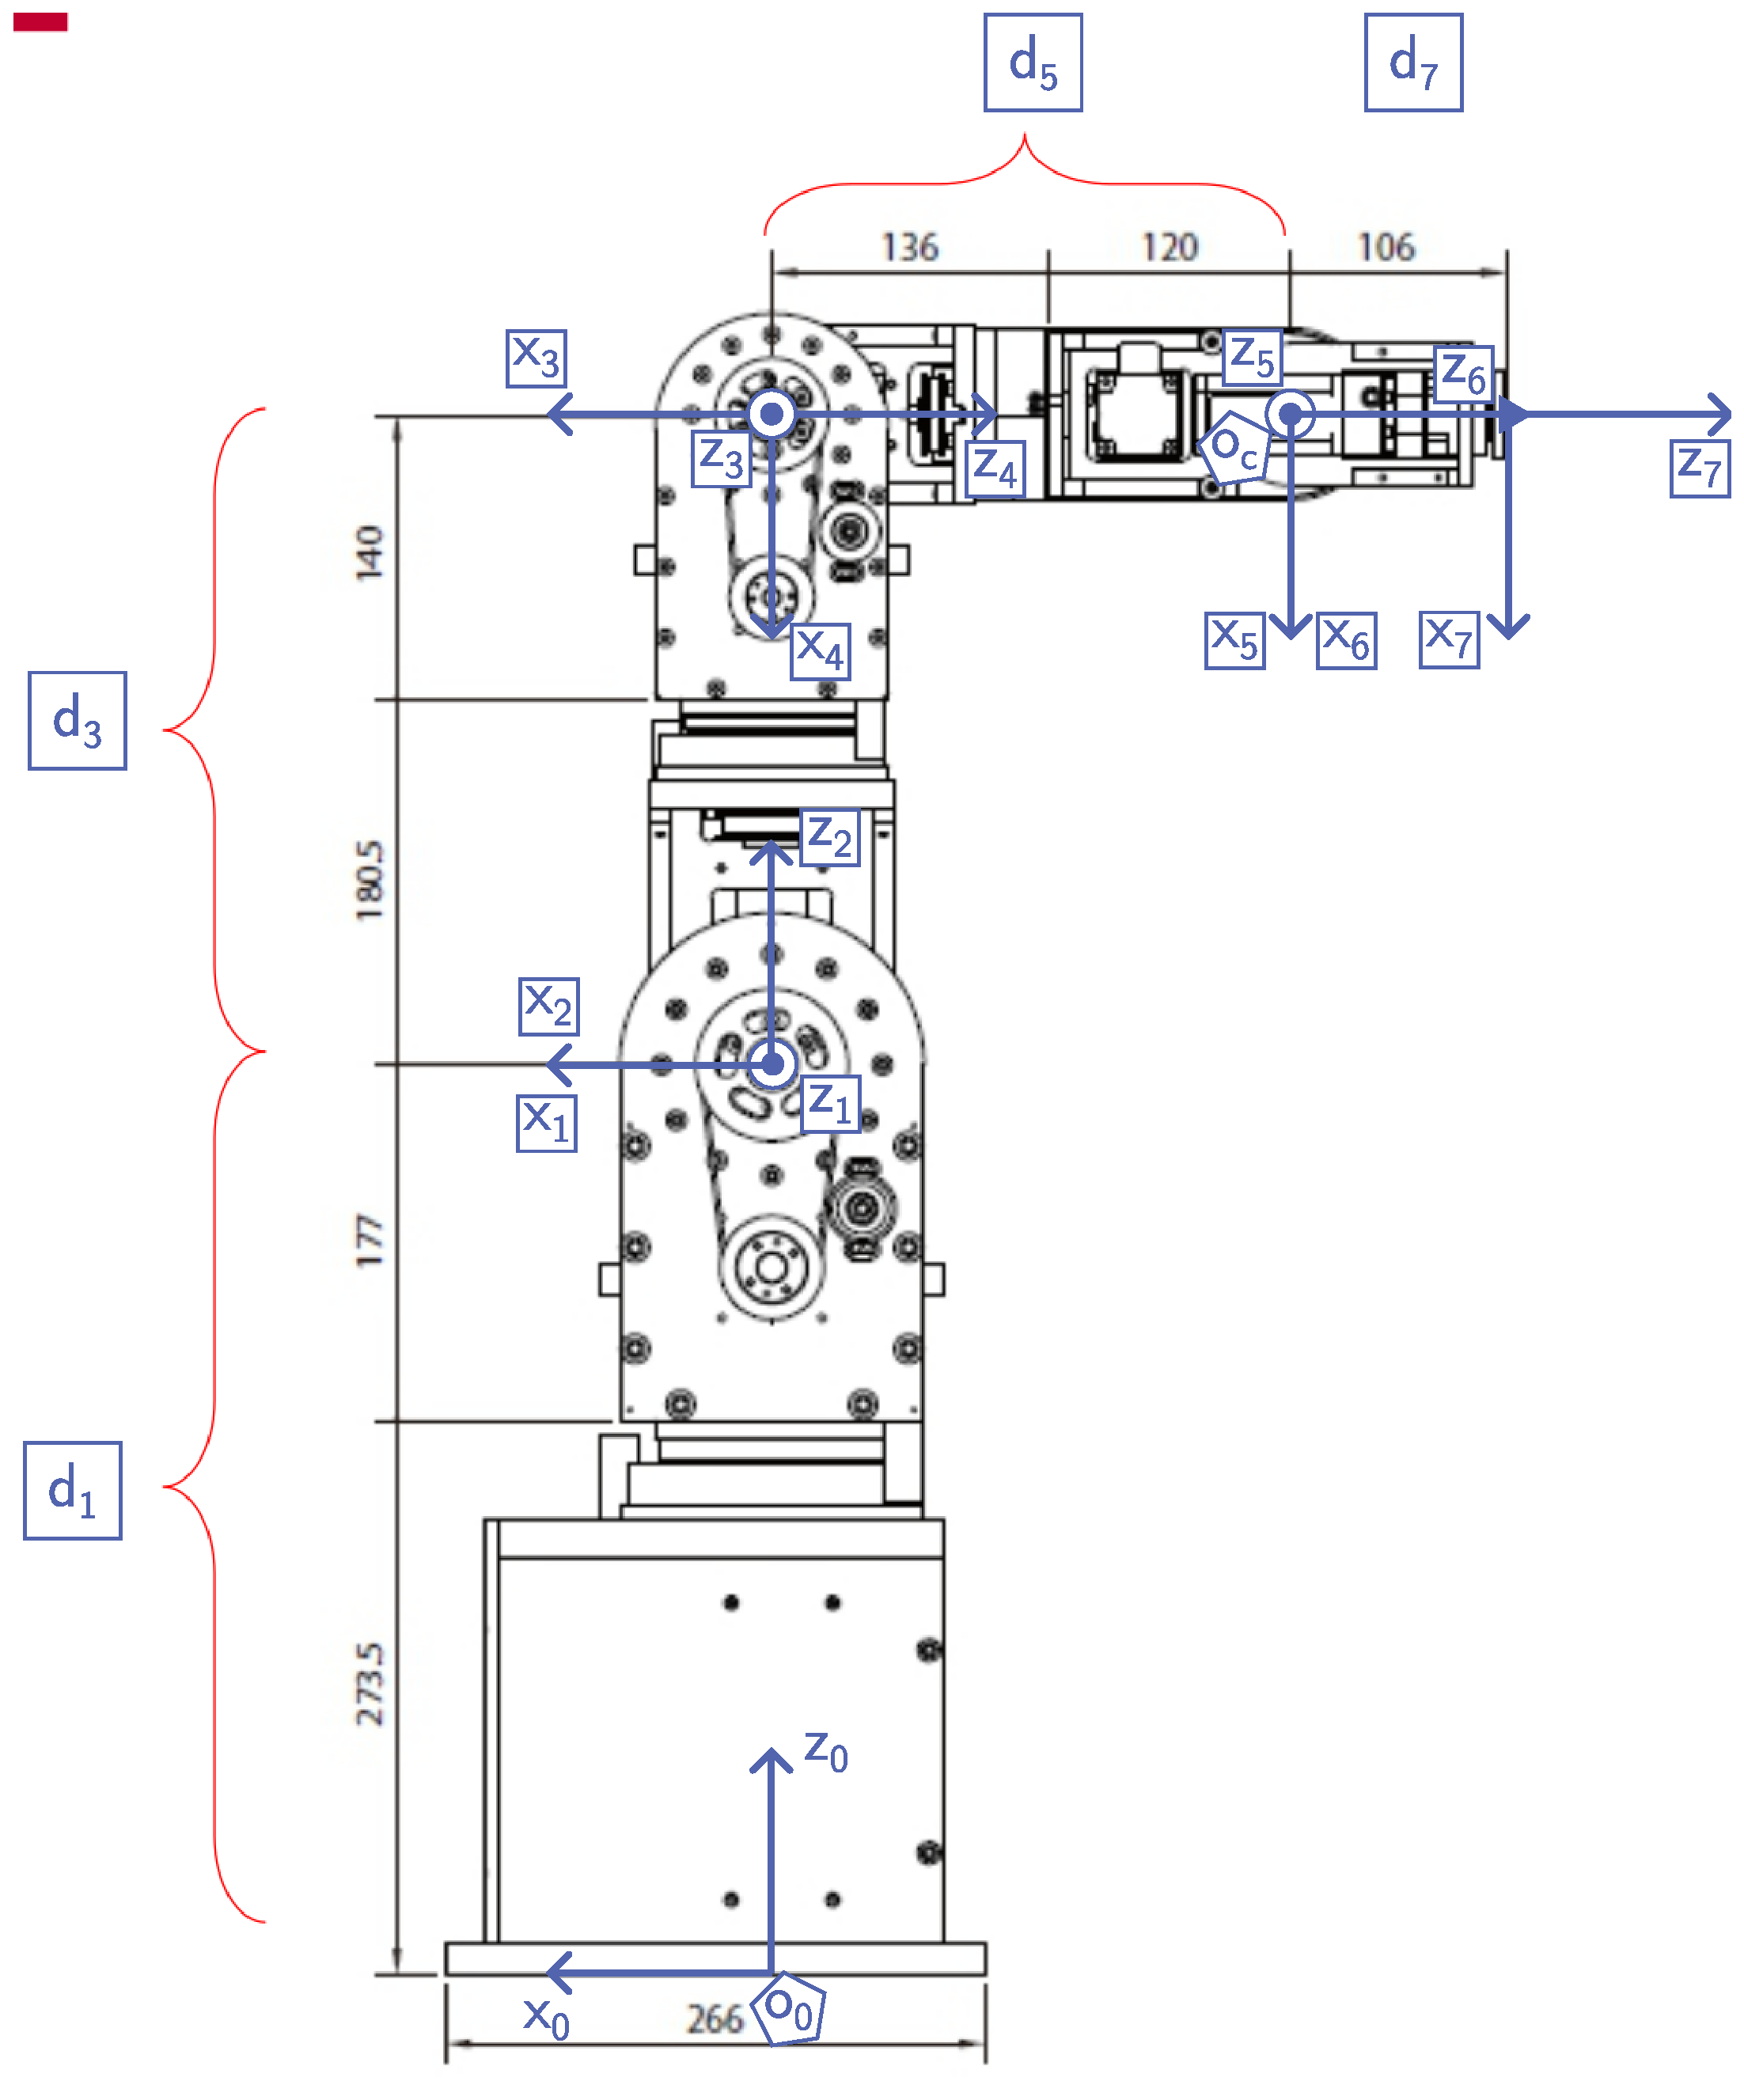
\includegraphics[width=0.5\textwidth]{./figures/minibot-7R.eps}
  \caption{Schematic of minibot-7R.}
  \label{fig:minibot}
\end{figure}

We will follow the classic Denavit-Hartenberg convention as presented 
in~\cite{spong2020robot}.

\section{Denavit-Hartenberg Formulation}
\label{sec:dh}

{\renewcommand{\arraystretch}{1.2}
\begin{table}[t]
    \caption{DH Table for minibot-7R}
    \label{tab:dh}
    \centering
    \begin{tabular}{ *5l }           \toprule
      \emph{Link}  & \emph{$\alpha_i$} [\unit{\degree}]& \emph{$a_i$} & \emph{$d_i$}\; [\unit{\milli\meter}] & \emph{$\theta_i$} [\unit{\degree}]\\ 
      \cmidrule(lr){1-1} \cmidrule(lr){2-2} \cmidrule(lr){3-3} \cmidrule(lr){4-4} \cmidrule(lr){5-5}
      $1$ & $-90$ & $0$ & $450.5$ & $\theta_1^*$ \\
    $2$ & $90$ & $0$ & $0$ & $\theta_2^*$ \\
    $3$ & $-90$ & $0$  & $320.5$ & $\theta_3^*$ \\
    $4$ & $-90$ & $0$ & $0$ & $\theta_4^*$ \\
    $5$ & $90$ & $0$ & $256$ & $\theta_5^*$ \\
    $6$ & $-90$ & $0$ & $0$ & $\theta_6^*$ \\
    $7$ & $0$ & $0$ & $106$ & $\theta_7^*$ \\ \midrule
    Home: & $\theta_i = 0^\circ$, & $i \neq 4$; & & $\theta_4 = 90^\circ$ \\
    \bottomrule
    \hline
    \end{tabular}
\end{table}
}

The transformation matrices between consecutive frames are given as follows.

\begin{align}
  \begin{split}
    A_1 &= \bmat{ c_1 & 0 & -s_1 & 0 \\ s_1 & 0 & c_1 & 0 \\ 0 & -1 & 0 & d_1 \\ 0 & 0 & 0 & 1}, \;\;
    A_2 = \bmat{ c_2 & 0 & s_2 & 0 \\ s_2 & 0 & -c_2 & 0 \\ 0 & 1 & 0 & 0 \\ 0 & 0 & 0 & 1}, \\
    A_3 &= \bmat{ c_3 & 0 & -s_3 & 0 \\ s_3 & 0 & c_3 & 0 \\ 0 & -1 & 0 & d_3 \\ 0 & 0 & 0 & 1}, \;\;
    A_4 = \bmat{ c_4 & 0 & -s_4 & 0 \\ s_4 & 0 & c_4 & 0 \\ 0 & -1 & 0 & 0 \\ 0 & 0 & 0 & 1}, \\
    A_5 &= \bmat{ c_5 & 0 & s_5 & 0 \\ s_5 & 0 & -c_5 & 0 \\ 0 & 1 & 0 & d_5 \\ 0 & 0 & 0 & 1}, \;\;
    A_6 = \bmat{ c_6 & 0 & -s_6 & 0 \\ s_6 & 0 & c_6 & 0 \\ 0 & -1 & 0 & 0 \\ 0 & 0 & 0 & 1}, \\
    A_7 &= \bmat{ c_7 & -s_7 & 0 & 0 \\ s_7 & c_7 & 0 & 0 \\ 0 & 0 & 1 & d_7 \\ 0 & 0 & 0 & 1}. \\
  \end{split}
\end{align}
%
The forward kinematics map is then given by \[ f: \mc{Q} \triangleq \prod_1^7
\mathbb{S}^1 \rightarrow \SEthree, \quad f(q) = \prod_1^7 A_i(q_i), \]
%
where $q_i = \theta_i$ are the joint variables.

An alternative assignment of frames is shown in Figure~\ref{fig:minibot_alt}
%
\begin{figure}[h]
  \centering
  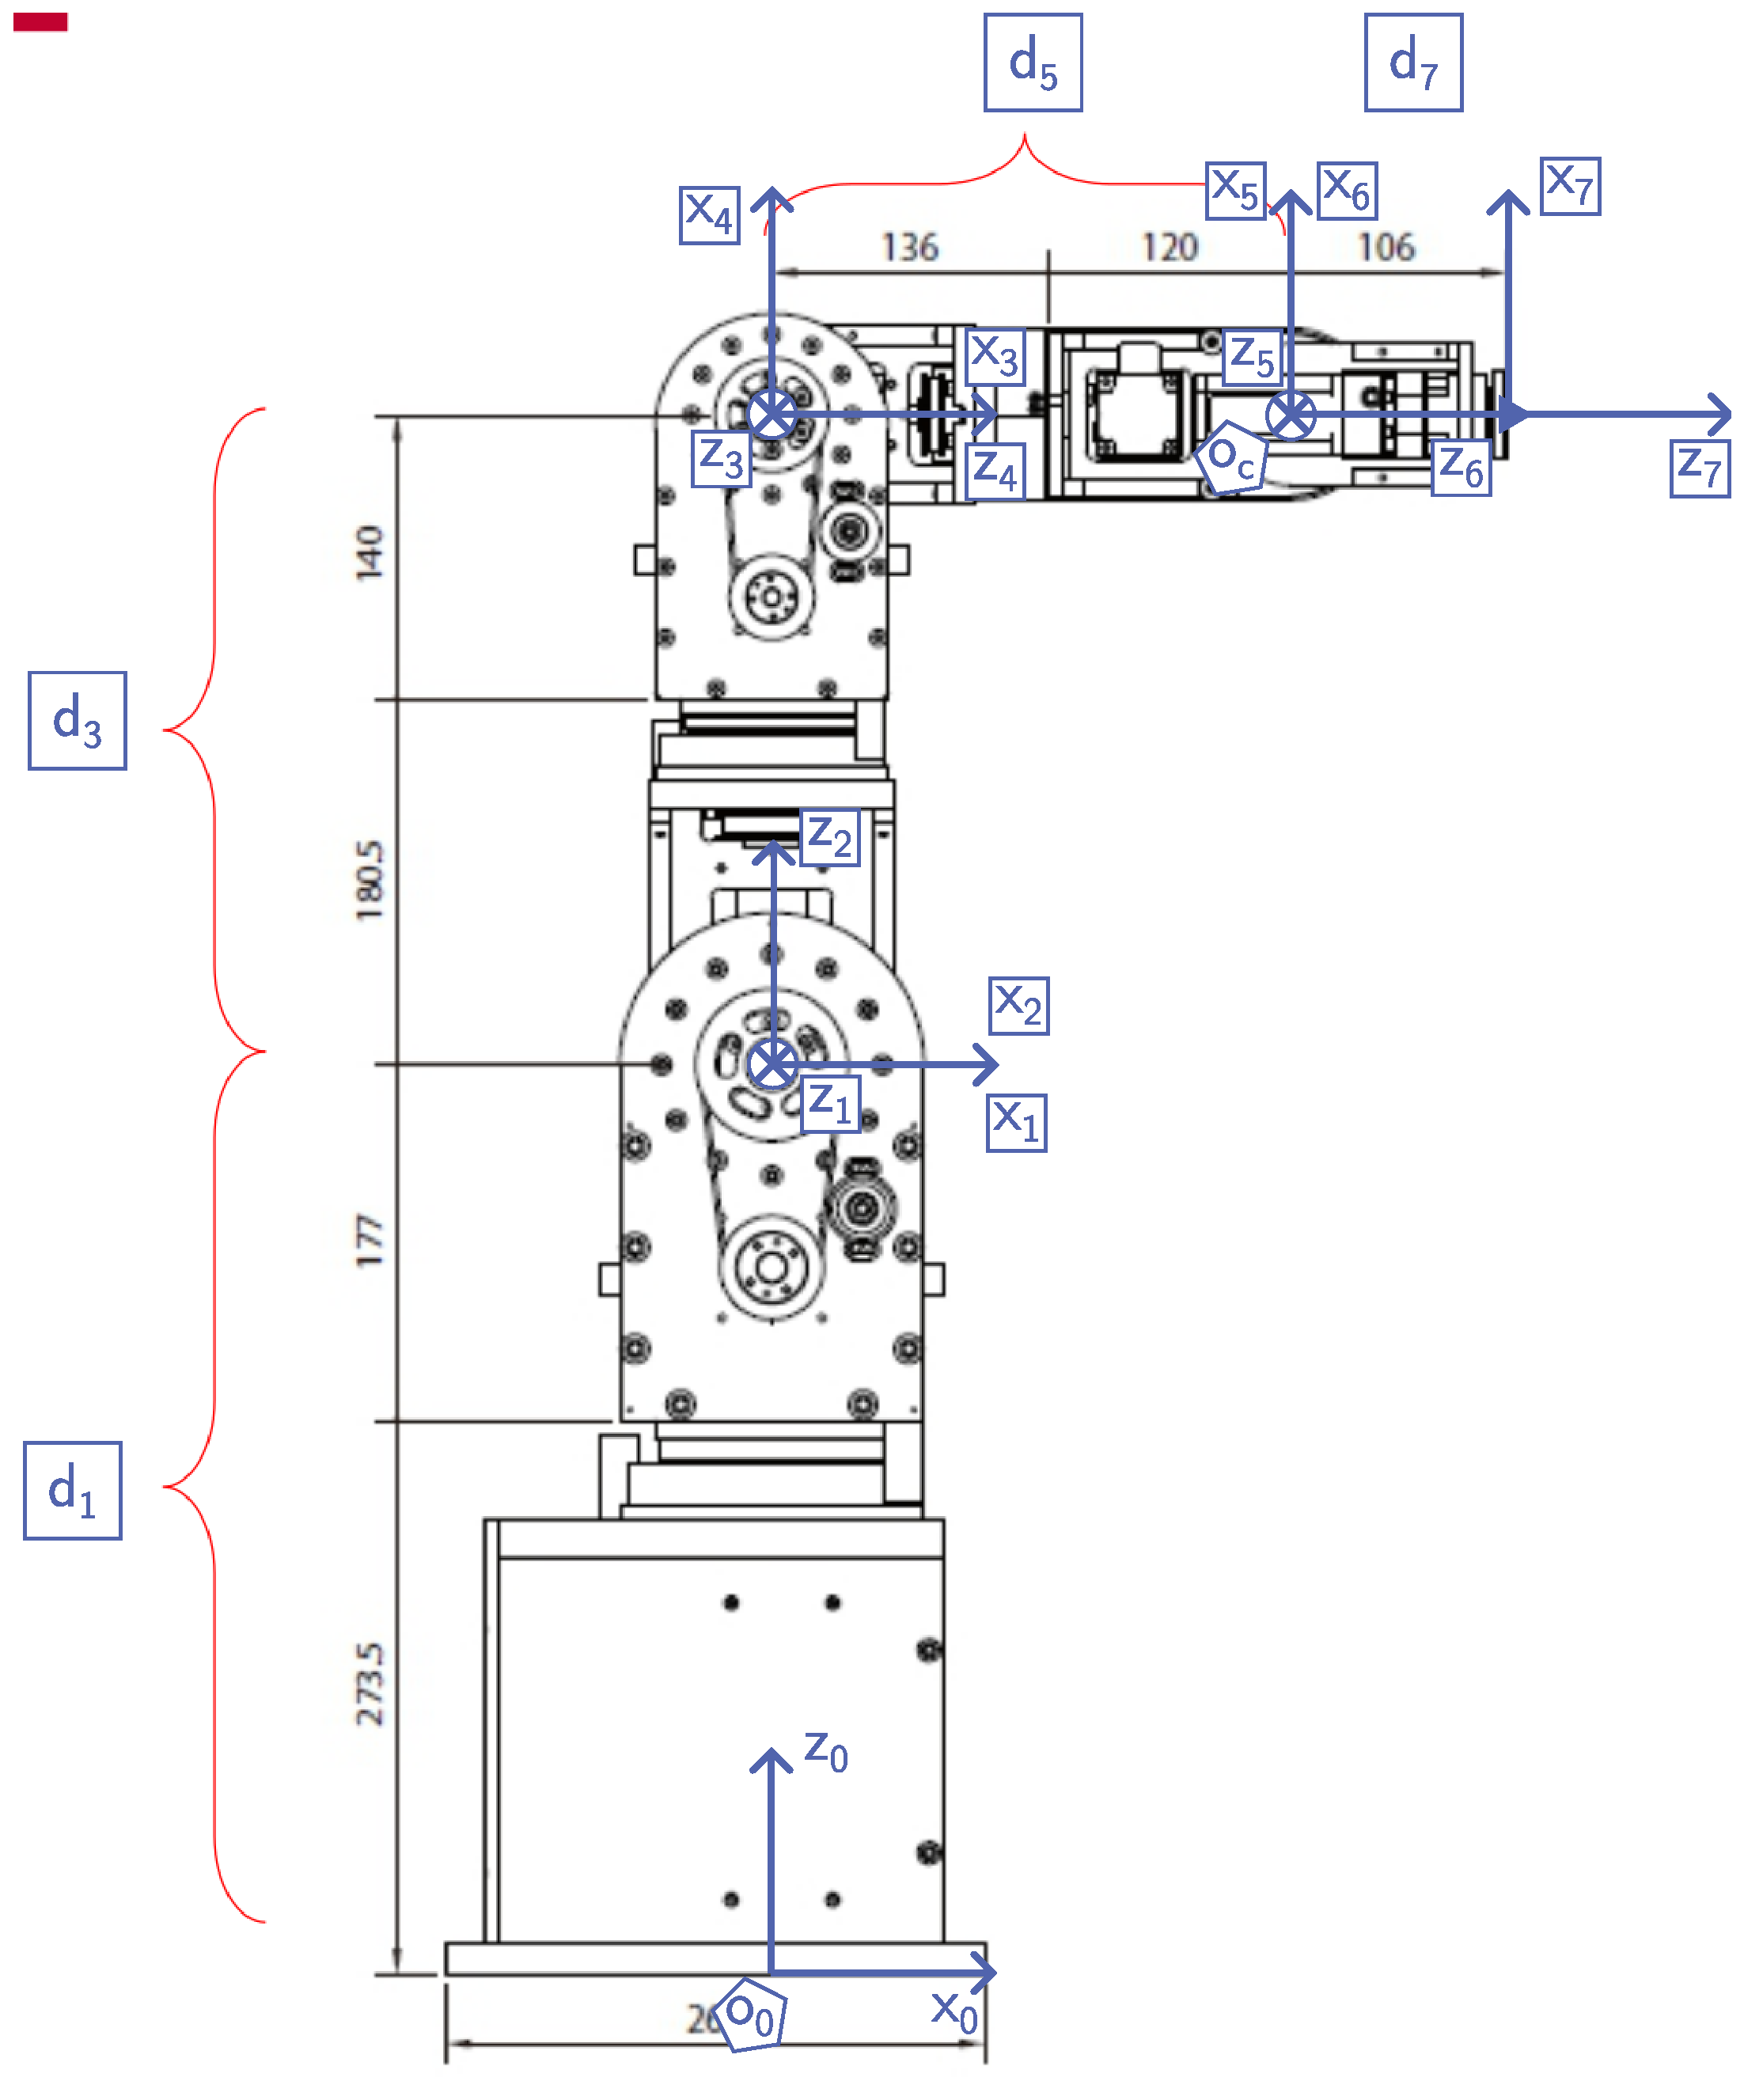
\includegraphics[width=0.5\textwidth]{./figures/minibot-7R_alternative.eps}
  \caption{Schematic of minibot-7R: Alternative DH frame assignment.}
  \label{fig:minibot_alt}
\end{figure}
%
When the frames are assigned in this way, the DH table~\ref{tab:dh} still
remains valid, except for the fact that the fact that at home position, we now
have $\theta_4 = -90^\circ$ rather than $90^\circ$.

\section{Velocity Kinematics}
\label{sec:vel}

We derive the Jacobian $\bm{J}: \mathbb{R}^7 \rightarrow \mathfrak{se}(3)$, that
maps the rate of change of the joint variables to the end effector twist.
This map can be represented in its matrix form by the concatenation of two 
submatrices, $\bm{J}_v$ and $\bm{J}_\omega$, as 
\begin{equation} 
  \bm{J} = \pmat{\bm{J}_v \\ \bm{J}_\omega}, 
  \label{eq:jac}
\end{equation}
where $\bm{J}_v$ and $\bm{J}_\omega$ are both elements of $\mathbb{R}^{3 \times
7}$. The construction of these matrices are subsequently shown, starting with 
$\bm{J}_v$.
%
\begin{align}
\begin{split}
  \bm{J}_v &= \bmat{\bm{J}_{v_1} & \bm{J}_{v_2} & \cdots & \bm{J}_{v_7}}, \\
  \bm{J}_{v_i} &= \bm{z}_{i-1} \times (\bm{o}_c - \bm{o}_{i-1}).
  \label{eq:jac_v}
\end{split}
\end{align}
%
The second part of the Jacobian matrix is constructed as 
\begin{equation}
  \bm{J}_\omega = \bmat{\bm{z}_0 & \bm{z}_1 & \cdots & \bm{z}_6}.
  \label{eq:jac_omega}
\end{equation}
%
With the Jacobian constructed as in~\eqref{eq:jac}, the end-effector 
twist $\bm{\xi} \in \mathfrak{se}(3)$ is related to the joint rates 
$\dot{\bm{q}} \in \mathbb{R}^7$ as \[ \bm{J} \dot{\bm{q}} = \bm{\xi}. \]

\section{Inverse Kinematics}
\label{sec:inversekin}

Suppose that we are given a point $H \in \SEthree$: 
\[ H = \bmat{R & o \\ 0 & 1}. \]
We want to find a $q \in \mc{Q}$ such that $f(q) = H$.

We first consider the inverse position kinematics problem, 
which assumes that the inverse orientation kinematics may be 
solved by using the final three joints, i.e., whatever the 
rotation matrix $^0R_4$ is, there exist $q_5$, $q_6$ and $q_7$, 
such that ${}^0R_4 {}^4R_7 = R$. The inverse position kinematics 
problem is then to find $q_1$ through $q_4$ such that the product $\prod_1^4
A_i$ has as its translation vector the wrist center location, $o_c \in
\mathbb{R}^3$.

In order to solve the inverse position problem, we first find the location of
the wrist center $o_c$ in the base coordinate system,
$\Sigma_0$: \[ o_c = o - d_7 R \bmat{0 \\ 0 \\ 1}. \]
%
We denote the current guess to the solution $q^d$ to the inverse position
kinematics problem by $q^{(k)}$ and perform the following iteration.

\begin{equation}
  q^{(k+1)} = q^{(k)} - \alpha_k M\left(q^{(k)}\right)\left(f\left(q^{(k)}\right) - o_c \right),
  \label{eq:ipk_iter}
\end{equation}
%
where the matrix $M$ could be taken as $\bar{J}_v^\dagger$ or $\bar{J}_v^\top$. 
$\bar{J}_v$ is the translation part of the Jacobian matrix that relates
$\dot{q}_1$ through $\dot{q}_4$ to the rate of change of the wrist center, i.e., 
$\bar{J}_v \dot{q}_{1:4} = \dot{o}_c$, where

\[ \bar{J}_v = \bmat{\bar{J}_{v_1} & \cdots & \bar{J}_{v_4}}, \]
where $\bar{J}_{v_{i+1}} = z_i \times (o_c - o_i)$, for $i = 0, \ldots 3$.


\bibliographystyle{ieeetr}        
\bibliography{./bib/references.bib}  



% \bibliographystyle{ieeetr}        
% \bibliography{../bib/references.bib}  

% \appendix

\noindent Recall from Section~\ref{sec:control} that the rms values of the
electric field in the transverse plane on a test point $q = (x, z)$ is given by
%
\begin{align*}
    \begin{split}
        \bar{E}_{x}^2(q) &=
        \frac{1}{2}\sum_{\alpha=1}^3\left(e_{\alpha}^2c_\alpha^2 -
            \sum_{\alpha^\prime > \alpha}^3e_{\alpha}
    e_{\alpha^\prime} c_{\alpha}c_{\alpha^\prime} \right), \\
        \bar{E}_{z}^2(q) &= \frac{1}{2}\sum_{\alpha=1}^3\left( e_{\alpha
            }^2s_\alpha^2 - \sum_{\alpha^\prime > \alpha}^3e_{\alpha}
    e_{\alpha^\prime} s_{\alpha}s_{\alpha^\prime}\right),
    \\
    \bar{E}^2 &= \frac{1}{2}\sum_{\alpha=1}^3\left(e_\alpha^2 -
    \sum_{\alpha^\prime > \alpha}^3 e_\alpha
    e_{\alpha^\prime} c_{\alpha \alpha^\prime}\right)
    \end{split}
\end{align*}
%
where $e_i$ and $\theta_i$ are the electric field peak magnitude and heading
angle from the $i^{\text{th}}$ wire to the test point $q$. 


\subsection{Derivatives}
\label{ssec:derivatives}

The following derivatives are needed in various applications of the chain rule.
%
\begin{equation*}
    \pd{\theta_\alpha}{x} = -\frac{1}{\xi}e_\alpha\sin{\theta_\alpha}, \quad
    \pd{\theta_\alpha}{z} = -\frac{1}{\xi}e_\alpha\cos{\theta_\alpha}.
\end{equation*}

\begin{equation*}
    \pd{e_\alpha}{x} = -\frac{1}{\xi}e_\alpha^2\cos{\theta_\alpha}, \quad
    \pd{e_\alpha}{z} = \frac{1}{\xi}e_\alpha^2\sin{\theta_\alpha}.
\end{equation*}

\begin{align*}
    \pd{\bar{E}_x^2}{e_\alpha} &= e_\alpha c_\alpha^2 -
    \frac{1}{2}\sum_{\alpha^\prime \neq \alpha}^3 e_{\alpha^\prime} c_\alpha
    c_{\alpha^\prime}, \\
    \pd{\bar{E}_z^2}{e_\alpha} &= e_\alpha s_\alpha^2 -
    \frac{1}{2}\sum_{\alpha^\prime \neq \alpha}^3 e_{\alpha^\prime} s_\alpha
    s_{\alpha^\prime}.
\end{align*}

\begin{align*}
    \pd{\bar{E}_x^2}{\theta_\alpha} &= -e_\alpha c_\alpha s_\alpha +
    \frac{1}{2}\sum_{\alpha^\prime \neq \alpha}^3 e_\alpha e_{\alpha^\prime}
    s_\alpha c_{\alpha^\prime}, \\
    \pd{\bar{E}_z^2}{\theta_\alpha} &= e_\alpha c_\alpha s_\alpha -
    \frac{1}{2}\sum_{\alpha^\prime \neq \alpha}^3 e_\alpha e_{\alpha^\prime}
    c_\alpha s_{\alpha^\prime}.
\end{align*}

\begin{align*}
    \pd{\bar{E}^2}{e_\alpha} &= e_\alpha - \frac{1}{2}\sum_{\alpha^\prime \neq
    \alpha} e_{\alpha^\prime}c_{\alpha \alpha^\prime},\\
    \pd{\bar{E}^2}{\theta_\alpha} &= \frac{1}{2} e_\alpha \sum_{\alpha^\prime \neq
\alpha} e_{\alpha^\prime} s_{\alpha \alpha^\prime}.
\end{align*}


\subsection{Gradients}
\label{ssec:gradients}
%
The Jacobian $J_{\bar{E}}$ is computed below using the chain rule.
\renewcommand*{\arraystretch}{1.5}
\[
    J_{\bar{E}}(q) = \bmat{ \pd{\bar{E}_x}{x}(q) & \pd{\bar{E}_x}{z}(q) \\
    \pd{\bar{E}_z}{x}(q) & \pd{\bar{E}_z}{z}(q)},
\]
%
The computation of this matrix is facilitated by the chain rule
%
\begin{align*}
    \pd{\bar{E}_x^2}{x} &= 2\bar{E}_x \pd{\bar{E}_x}{x} = \sum_{\alpha=1}^3
    \left(\pd{\bar{E}_x^2}{e_\alpha}\pd{e_\alpha}{x} +
    \pd{\bar{E}_x^2}{\theta_\alpha}\pd{\theta_\alpha}{x}\right), \\
    \pd{\bar{E}_x^2}{z} &= 2\bar{E}_x \pd{\bar{E}_x}{z} =\sum_{\alpha=1}^3
    \left(\pd{\bar{E}_x^2}{e_\alpha}\pd{e_\alpha}{z} +
    \pd{\bar{E}_x^2}{\theta_\alpha}\pd{\theta_\alpha}{z}\right), \\
    \pd{\bar{E}_z^2}{x} &= 2\bar{E}_z \pd{\bar{E}_z}{x} = \sum_{\alpha=1}^3
    \left(\pd{\bar{E}_z^2}{e_\alpha}\pd{e_\alpha}{x} +
    \pd{\bar{E}_z^2}{\theta_\alpha}\pd{\theta_\alpha}{x}\right), \\
    \pd{\bar{E}_z^2}{z} &= 2\bar{E}_z \pd{\bar{E}_z}{z} = \sum_{\alpha=1}^3
    \left(\pd{\bar{E}_z^2}{e_\alpha}\pd{e_\alpha}{z} +
    \pd{\bar{E}_z^2}{\theta_\alpha}\pd{\theta_\alpha}{z}\right), \\
    \pd{\bar{E}^2}{x} &= 2\bar{E} \pd{\bar{E}}{x} = \sum_{\alpha=1}^3
    \left(\pd{\bar{E}^2}{e_\alpha}\pd{e_\alpha}{x} +
    \pd{\bar{E}^2}{\theta_\alpha}\pd{\theta_\alpha}{x}\right), \\
    \pd{\bar{E}^2}{z} &= 2\bar{E} \pd{\bar{E}}{z} = \sum_{\alpha=1}^3
    \left(\pd{\bar{E}^2}{e_\alpha}\pd{e_\alpha}{z} +
    \pd{\bar{E}^2}{\theta_\alpha}\pd{\theta_\alpha}{z}\right).
\end{align*}
%


\subsection{Hessian}
\label{ssec:hessian}

\noindent We compute the Hessian of $H_{\bar{E}}(q) = \nabla_q^2 \bar{E}(q)$ of
$\bar{E}$. First, note the identities

\begin{align*}
    \pd{}{x}\pd{\bar{E}^2}{x} &= \pd{}{x}\left( 2\bar{E}\pd{\bar{E}}{x} \right) =
    2\left(\pd{\bar{E}}{x}\right)^2 + 2\bar{E}\pdd{\bar{E}}{x} \\
&\Rightarrow \pdd{\bar{E}}{x} = \frac{1}{2\bar{E}} \pdd{\bar{E}^2}{x} -
\frac{1}{\bar{E}}\left(\pd{\bar{E}}{x}\right)^2. \\
    \pd{}{z}\left(\pd{\bar{E}^2}{x}\right) &=
    \pd{}{z}\left(2\bar{E}\pd{\bar{E}}{x}\right) =
    2\pd{\bar{E}}{z}\pd{\bar{E}}{x} + 2\bar{E}\frac{\partial^2 \bar{E}}{\partial
    z \partial x} \\
&\Rightarrow \frac{\partial^2 \bar{E}}{\partial z \partial x} = \frac{\partial^2
\bar{E}}{\partial x \partial z} = \frac{1}{2\bar{E}} \frac{\partial^2
\bar{E}^2}{\partial z \partial x} - \frac{1}{\bar{E}}
\pd{\bar{E}}{z}\pd{\bar{E}}{x}. \\
\pd{}{z}\pd{\bar{E}^2}{z} &= \pd{}{z}\left( 2\bar{E}\pd{\bar{E}}{z} \right) =
    2\left(\pd{\bar{E}}{z}\right)^2 + 2\bar{E}\pdd{\bar{E}}{z} \\
&\Rightarrow \pdd{\bar{E}}{z} = \frac{1}{2\bar{E}} \pdd{\bar{E}^2}{z} -
\frac{1}{\bar{E}}\left(\pd{\bar{E}}{z}\right)^2.
\end{align*}
%
We now compute the second derivatives
%
\begin{align*}
    &\xi^2 \pdd{\bar{E}^2}{x} = \sum_{\alpha=1}^3 \left[e_\alpha^4 \left(1 +
    2\cos{(2\theta_\alpha)}\right) - \right. \\ 
    &\phantom{13}\left. \sum_{\alpha^\prime \neq \alpha} e_\alpha
e_{\alpha^\prime}^3 \cos{(\theta_\alpha - 3\theta_{\alpha^\prime})} -
\sum_{\alpha^\prime > \alpha} e_\alpha^2 e_{\alpha^\prime}^2 \cos{(2\theta_\alpha
- \theta_{\alpha^\prime})}\right], \\
   &\xi^2 \frac{\partial^2 \bar{E}^2}{\partial z \partial x} = \xi^2
   \frac{\partial^2 \bar{E}^2}{\partial x \partial z} = \\
   &\phantom{123}\sum_{\alpha=1}^3
   \left( -2e_\alpha^4\sin{2\theta_\alpha} - \sum_{\alpha^\prime \neq \alpha}
   e_\alpha e_{\alpha^\prime}^3 \sin{(\theta_\alpha -
3\theta_{\alpha^\prime})}\right), \\
&\xi^2 \pdd{\bar{E}^2}{z} = \sum_{\alpha=1}^3 \left[e_\alpha^4 \left(1 -
    2\cos{(2\theta_\alpha)}\right) + \right. \\ 
    &\phantom{13}\left. \sum_{\alpha^\prime \neq \alpha} e_\alpha
e_{\alpha^\prime}^3 \cos{(\theta_\alpha - 3\theta_{\alpha^\prime})} -
\sum_{\alpha^\prime > \alpha} e_\alpha^2 e_{\alpha^\prime}^2 \cos{(2\theta_\alpha
- \theta_{\alpha^\prime})}\right].
\end{align*}

With these computations the Hessian matrix is given by 
%
\begin{equation*}
    H_{\bar{E}}(q) = \bmat{
        \pdd{\bar{E}}{x} & \frac{\partial^2 \bar{E}}{\partial z \partial x} \\
        \frac{\partial^2 \bar{E}}{\partial x \partial z} & \pdd{\bar{E}}{z}
    }.
\end{equation*}


\subsection{Potential Function}
\label{ssec:potfcn}

We define the potential function $V(q) \triangleq \nicefrac{1}{\bar{E}(q)^2}$. This
is a decreasing function of $\bar{E}$. Its various derivatives satisfy the
identities.

\begin{equation*}
    \pd{V}{x}(q) = -\dfrac{2}{\bar{E}^3}\pd{\bar{E}}{x}, \qquad 
    \pd{V}{z}(q) = -\dfrac{2}{\bar{E}^3}\pd{\bar{E}}{z}.
\end{equation*}

\begin{align*}
    \pdd{V}{x} &= \dfrac{6}{\bar{E}^4}\left( \pd{\bar{E}}{x} \right)^2 -
    \frac{2}{\bar{E}^3}\pdd{\bar{E}}{x}, \\
    \frac{\partial^2 V}{\partial z \partial x} &= \frac{\partial^2 V}{\partial x
    \partial z} = \dfrac{6}{\bar{E}^4}\left( \pd{\bar{E}}{z} \pd{\bar{E}}{x}
    \right) - \frac{2}{\bar{E}^3}\frac{\partial^2 \bar{E}}{\partial z \partial
    x}, \\
    \pdd{V}{z} &= \dfrac{6}{\bar{E}^4}\left( \pd{\bar{E}}{z} \right)^2 -
    \frac{2}{\bar{E}^3}\pdd{\bar{E}}{z}.
\end{align*}

The Hessian of the potential function is given by 
\begin{equation*}
    H_{V}(q) = \bmat{
        \pdd{V}{x} & \frac{\partial^2 V}{\partial z \partial x} \\
        \frac{\partial^2 V}{\partial x \partial z} & \pdd{V}{z}
    }.
\end{equation*}

% 
% \vspace{9em}
% 
% \begin{IEEEbiography}[{\includegraphics[width=1in,height=1.25in,clip,keepaspectratio]{siric.jpg}}]
%     %
%     {Wankun Sirichotiyakul} (M'21) was born in Bangkok, Thailand. He received
%     the B.Sc. (2017) and M.Sc. (2019) degrees in mechanical engineering from
%     Boise State University, Boise, Idaho, USA, where he is currently working
%     toward the Ph.D. degree in electrical and computer engineering. 
%     
%     His research interests are in the intersection of optimization and machine
%     learning approaches to the control of robotic systems.
% \end{IEEEbiography}
% 
% \begin{IEEEbiography}[{\includegraphics[width=1in,height=1.25in,clip,keepaspectratio]{ashen.jpg}}]
%     %
%     {Nardos A. Ashenafi} (M'21) was born and raised in Ethiopia. She came to the
%     United States to further her education in the field of engineering,
%     robotics, and control. She received the B.Sc degree in mechanical
%     engineering (2019) and the M.Engr degree in electrical engineering (2021)
%     from Boise State University, Idaho, USA. She is currently pursuing the Ph.D.
%     degree in electrical and computer engineering at Boise State University with
%     emphasis in robotics and control of dynamical systems. 
%     
%     Her interests include mechanical design, nonlinear
%     control, machine learning and mechatronics.
% \end{IEEEbiography}
% 
% \begin{IEEEbiography}[{\includegraphics[width=1in,height=1.25in,clip,keepaspectratio]{satic.jpg}}]
%     %
%     {AYKUT C. SATICI} (M'12) received the B.Sc. and M.Sc. degrees in
%     mechatronics engineering from Sabanci University, Istanbul, Turkey, in
%     2008 and 2010, respectively, and the Master's degree in mathematics from
%     the University of Texas, Dallas, TX, USA, in 2013. He received his Ph.D.
%     degree from the Electrical Engineering Department, University of Texas at
%     Dallas. 
% 
%     He is currently with the Boise State University where he is an assistant
%     professor of Mechanical and Biomedical Engineering. He has authored or
%     co-authored more than 30 technical papers in control and robotics. His
%     current research interests include robotics, geometric mechanics,
%     nonlinear control theory, and machine learning for robotics.
%     
%     Dr. Satici has been serving an Associate Editor for the International
%     Conference on Robotics and Automation for 3 years and is in the Program
%     Committee for American Control Conference 2023.
% \end{IEEEbiography}
% 
% \vspace{20.5em}

\end{document}
